\documentclass[11pt,twocolumn]{article}

\usepackage[utf8]{inputenc}
\usepackage[T1]{fontenc}
% Using default Computer Modern fonts
\usepackage{amsmath,amssymb,amsfonts}
\usepackage{graphicx}
\usepackage{hyperref}
\usepackage[margin=2cm]{geometry}
\usepackage{booktabs}
\usepackage{xcolor}
\usepackage{listings}
\usepackage{enumitem}
\usepackage{cite}
\usepackage{url}
\usepackage{tikz}
\usetikzlibrary{arrows.meta,positioning,shapes.geometric,calc,fit}

\hypersetup{
  colorlinks=true,
  linkcolor=blue!60!black,
  citecolor=blue!60!black,
  urlcolor=blue!60!black,
  pdftitle={BSVM: A Validity-Proven EVM Layer 2 on BSV via Covenant UTXO Chains and STARK Proofs},
  pdfauthor={Siggi Oskarsson},
  pdfsubject={Ethereum Virtual Machine Layer 2 on BSV with STARK validity proofs},
  pdfkeywords={EVM, Layer 2, BSV, STARK, zero-knowledge proofs, covenant, UTXO, zkVM, SP1, rollup},
  pdfcreator={LaTeX with hyperref},
  pdfproducer={BSVM Project},
  bookmarks=true,
  bookmarksnumbered=true
}

\lstset{
  basicstyle=\ttfamily\footnotesize,
  breaklines=true,
  frame=single,
  xleftmargin=1em,
  framexleftmargin=0.5em,
  numbers=none,
  columns=flexible
}

\title{\textbf{BSVM: A Validity-Proven EVM Layer~2 on Bitcoin~SV\\via Covenant UTXO Chains and STARK Proofs}}

\author{
Siggi \'{O}skarsson \\
\textit{BSV Association} \\
\texttt{siggi.oskarsson@bsvassociation.org}
}

\date{April 2026}

\begin{document}

\twocolumn[
\begin{@twocolumnfalse}
\maketitle
\begin{abstract}
We present BSVM, a Layer~2 Ethereum Virtual Machine that runs on Bitcoin~SV (BSV) as its settlement and data availability layer. BSVM achieves full EVM bytecode compatibility while anchoring every state transition to BSV through a novel \emph{covenant UTXO chain} architecture. Each L2 state advance is a BSV transaction that spends a covenant-locked UTXO and creates a new one, forming a chain of state commitments enforced by Bitcoin Script. State transition correctness is guaranteed by STARK validity proofs generated via the SP1 zero-knowledge virtual machine, which proves the execution of a Rust EVM interpreter (revm) compiled to RISC-V. The covenant verifies the proof on-chain via one of three R\'{u}nar-compiled modes: native STARK verification using a FRI verifier over the KoalaBear field with on-chain Poseidon2 Merkle openings (Mode~1, transparent, no trusted setup, $\sim$1.2\,MB proof, $\sim$849\,KB locking script for the evm-guest preset), or SP1's Groth16/BN254 wrap verified via on-chain BN254 pairing (Modes~2 and 3, $\sim$256-byte proof, $\sim$400\,ms verification); Mode~3 uses a witness-assisted verifier with the SP1 verifying key baked into an inlined preamble and is the recommended production target. The system requires no privileged sequencer key---the proof alone authorizes state advances, meaning anyone with a valid proof can advance the chain. BSVM supports an ecosystem of independent EVM instances (\emph{shards}), each with its own covenant chain and node network. At a BSV fee rate of 100~sat/KB, a 128-transaction batch under Mode~3 costs approximately 21,600~satoshis to post on-chain ($\approx$\$0.0065), yielding a per-transaction L1 cost of 169~satoshis ($\approx$\$0.00005); Modes~1 and 2 carry larger per-advance footprints and correspondingly higher L1 cost. We describe the architecture, proof pipeline, fee model, bridge design, and security properties in full.
\end{abstract}
\vspace{1em}
\end{@twocolumnfalse}
]

% ─────────────────────────────────────────────
\section{Introduction}
\label{sec:intro}

The Ethereum Virtual Machine (EVM) has emerged as the dominant smart contract execution environment, with over \$100B in total value locked across EVM-compatible chains as of 2025~\cite{l2beat}. However, Ethereum's Layer~1 gas costs remain prohibitive for many applications, driving demand for Layer~2 (L2) solutions that execute transactions off-chain while inheriting L1 security guarantees.

Existing L2 architectures---optimistic rollups~\cite{arbitrum,optimism} and zero-knowledge rollups~\cite{zksync,scroll,polygon_zkevm}---all build on Ethereum as their L1. This creates a dependency on Ethereum's limited throughput and volatile fee market. When Ethereum L1 gas prices spike, L2 posting costs increase proportionally, as L2s must compete for Ethereum block space to publish batch data and proofs.

We observe that the ideal L1 for an EVM L2 has three properties: (1)~large or unbounded data capacity for cheap batch posting, (2)~stable and predictable fees, and (3)~a UTXO model amenable to covenant-based state locking. Bitcoin~SV (BSV)~\cite{bsv_scaling} satisfies all three. BSV allows unbounded transaction and block sizes, charges a stable fee rate of approximately 100~satoshis per kilobyte, and supports advanced Bitcoin Script operations including introspection opcodes that enable covenant contracts~\cite{runar}.

BSVM leverages these properties to build an EVM L2 that is:

\begin{itemize}[nosep,leftmargin=1.5em]
\item \textbf{Fully EVM-compatible}: Existing Solidity contracts, MetaMask, ethers.js, Hardhat, and Foundry work without modification.
\item \textbf{Validity-proven}: Every state transition is proven correct by a STARK proof covering full EVM execution---every opcode, every state access, every balance transfer.
\item \textbf{Sequencer-free}: No privileged key can advance the state. The STARK proof is the sole authorization. Anyone with a valid proof can advance the covenant.
\item \textbf{Extremely cheap}: At 100~sat/KB, a 128-transaction batch costs $\approx$21,600~sats ($\approx$\$0.0065) on L1, yielding per-transaction costs of $\approx$\$0.00005.
\end{itemize}

The remainder of this paper is organized as follows. Section~\ref{sec:background} reviews relevant background. Section~\ref{sec:architecture} presents the overall system architecture. Section~\ref{sec:evm} describes the EVM extraction and execution engine. Section~\ref{sec:proofs} details the validity proof pipeline. Section~\ref{sec:covenant} describes the covenant contract and on-chain verification. Section~\ref{sec:fees} analyzes the fee model and prover economics. Section~\ref{sec:bridge} presents the bridge design. Section~\ref{sec:security} provides a security analysis. Section~\ref{sec:related} discusses related work, and Section~\ref{sec:conclusion} concludes.

% ─────────────────────────────────────────────
\section{Background}
\label{sec:background}

\subsection{The Ethereum Virtual Machine}

The EVM is a stack-based, 256-bit word-size virtual machine that executes smart contract bytecode~\cite{wood_ethereum}. It operates over a world state organized as a Merkle Patricia Trie (MPT)~\cite{wood_ethereum}, where each account's storage is itself a trie. The EVM's gas metering system ensures execution terminates and provides a fee mechanism. Modern EVM implementations support the full hardfork history from Frontier through Prague, including EIP-1559 fee markets~\cite{eip1559}, EIP-2929 access lists~\cite{eip2929}, and EIP-1153 transient storage~\cite{eip1153}.

\subsection{BSV and Unbounded Blocks}

Bitcoin~SV restores the original Bitcoin protocol~\cite{nakamoto} with no artificial limits on transaction or block size~\cite{bsv_scaling}. Key properties relevant to BSVM:

\begin{itemize}[nosep,leftmargin=1.5em]
\item \textbf{Unbounded OP\_RETURN}: Transactions can carry arbitrary data payloads, enabling cheap L2 data availability.
\item \textbf{Unlimited unconfirmed chain depth}: BSV allows arbitrarily long chains of unconfirmed transactions, each spending the output of the previous. BTC limits this to $\approx$25 transactions.
\item \textbf{Stable fees}: BSV maintains a fee rate of approximately 100~sat/KB, independent of network demand.
\item \textbf{Script expressiveness}: BSV's Script supports arithmetic, hashing, and introspection opcodes (e.g., OP\_PUSH\_TX for sighash preimage access) that enable covenant contracts.
\end{itemize}

\subsection{Covenant Contracts}

A \emph{covenant} is a Bitcoin locking script that constrains how the output may be spent, including constraints on the spending transaction's outputs~\cite{moser_covenants}. Using OP\_PUSH\_TX (which provides the sighash preimage to Script), a covenant can inspect the spending transaction's outputs and enforce that specific output scripts and values are maintained. This enables \emph{stateful UTXO chains}: a UTXO is spent and recreated with updated state data, forming a deterministic chain of state transitions anchored in BSV's blockchain.

\subsection{STARK Proofs}

Scalable Transparent Arguments of Knowledge (STARKs)~\cite{ben_sasson_stark} are proof systems based on hash functions and polynomial commitments via the FRI protocol~\cite{ben_sasson_fri}. Unlike SNARKs~\cite{groth16}, STARKs require no trusted setup and are conjectured post-quantum secure. STARK verification involves checking polynomial evaluations against Merkle commitments---operations that decompose into hash computations and field arithmetic, making them amenable to verification in resource-constrained environments such as Bitcoin Script. SP1 additionally offers an optional Groth16 \emph{wrapper}: the STARK is recursively verified inside a BN254 Groth16 circuit, producing a $\sim$256-byte SNARK proof that can be checked by a single BN254 pairing equation~\cite{groth16}. The wrapper reintroduces a BN254 trusted-setup assumption but dramatically reduces on-chain verification cost relative to native FRI verification, and BSVM exposes both options as separate covenant modes.

\subsection{Zero-Knowledge Virtual Machines}

A zero-knowledge virtual machine (zkVM) proves the correct execution of arbitrary programs. SP1~\cite{sp1} is a STARK-based zkVM that proves RISC-V program execution. Programs are compiled from Rust (or any LLVM-compiled language) to RISC-V ELF binaries. SP1 includes \emph{precompiles}---optimized circuits for common operations such as keccak256 and secp256k1---that reduce proving cost by 5--10$\times$ compared to naive RISC-V execution~\cite{sp1}. SP1 is audited by four firms and secures over \$1B in total value locked across production systems~\cite{sp1}.

\subsection{The R\'{u}nar Compiler}

R\'{u}nar~\cite{runar} is a multi-language Bitcoin Script compiler with independent implementations in Go, TypeScript, Rust, and Python that produce byte-identical output via an Administrative Normal Form (ANF) intermediate representation. R\'{u}nar provides a domain-specific language for writing covenant contracts that compile to Bitcoin Script. The multi-implementation conformance property---all compilers producing identical output for the same contract---provides formal correctness assurance that is critical for a covenant guarding L2 state.

% ─────────────────────────────────────────────
\section{System Architecture}
\label{sec:architecture}

\subsection{Overview}

BSVM is an ecosystem of independent EVM instances (\emph{shards}), each running as a BSV overlay network. Each shard consists of:

\begin{enumerate}[nosep,leftmargin=1.5em]
\item A \textbf{covenant UTXO chain} on BSV: a sequence of BSV transactions, each spending the previous covenant UTXO, forming the canonical state commitment chain.
\item A \textbf{node network}: multiple nodes that replicate state via peer-to-peer gossip, execute EVM transactions deterministically, and race to generate STARK proofs and advance the covenant.
\item A \textbf{bridge covenant}: one or more BSV UTXOs that hold locked BSV backing the shard's native token (wBSV).
\end{enumerate}

There is no centralized sequencer. BSV is the consensus layer---whichever node successfully spends the covenant UTXO first determines the canonical state for that batch. Other nodes accept the winner's ordering by replaying the batch data from BSV.

\subsection{Multi-Shard Model}

Shards are sovereign and independent. A DeFi project launches its own shard with its own chain ID, contract deployments, and covenant chain. An identity project launches a separate shard. Cross-shard interaction is asynchronous bridging---lock on one shard, mint on another---analogous to bridging between Ethereum and Arbitrum. Within a shard, full Ethereum-style atomic composability (cross-contract calls) is supported.

\subsection{Covenant UTXO Chain}

The core data structure is a chain of BSV transactions, each spending the previous covenant output:

\begin{center}
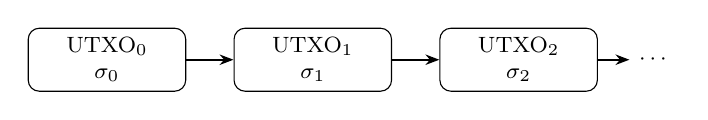
\begin{tikzpicture}[
  node distance=0.6cm,
  box/.style={draw, rounded corners, minimum width=2cm, minimum height=0.8cm, font=\footnotesize, align=center},
  arr/.style={-{Stealth[length=5pt]}, thick}
]
\node[box] (u0) {UTXO$_0$\\$\sigma_0$};
\node[box, right=of u0] (u1) {UTXO$_1$\\$\sigma_1$};
\node[box, right=of u1] (u2) {UTXO$_2$\\$\sigma_2$};
\node[right=0.4cm of u2, font=\footnotesize] (dots) {$\cdots$};
\draw[arr] (u0) -- (u1);
\draw[arr] (u1) -- (u2);
\draw[arr] (u2) -- (dots);
\end{tikzpicture}
\end{center}

\noindent Each UTXO$_i$ carries a compact 41-byte state tuple in its locking script: the 32-byte EVM state root $r_i$ (Merkle Patricia Trie root of the EVM world state), the 8-byte block number $i$, and a 1-byte frozen flag used by governance (see \S\ref{sec:security}). Bridge-specific commitments---cumulative deposit counter, withdrawal-nullifier commitment chain, and bridge nonce for replay protection---live in independent sub-covenant UTXOs (\S\ref{sec:bridge}) rather than the state covenant, keeping the per-advance hot path small. The chain ID is baked into the locking script as a compile-time constant so every advance is implicitly shard-scoped. The locking script is a R\'{u}nar-compiled covenant that verifies a validity proof before allowing the spend, and emits the batch data in an OP\_RETURN output whose inclusion is cryptographically enforced by the covenant's continuation-hash commitment (\S\ref{sec:covenant}). BSV's unlimited unconfirmed chain depth allows hundreds or thousands of covenant advances between BSV blocks. When a block is mined, the entire chain is confirmed atomically.

\subsection{Transaction Flow}

A user submits a signed EVM transaction via \texttt{eth\_sendRawTransaction} (standard Ethereum RPC). The overlay node:

\begin{enumerate}[nosep,leftmargin=1.5em]
\item Validates the transaction (signature, nonce, gas, balance).
\item Executes it through the Go EVM engine (sub-millisecond).
\item Returns the receipt immediately.
\item Batches the transaction with up to 127 others.
\item Generates a STARK proof of the batch via SP1.
\item Builds a BSV transaction spending the covenant UTXO, with the proof in the unlocking script and batch data in an OP\_RETURN output.
\item Broadcasts the BSV transaction.
\end{enumerate}

The user receives a receipt in milliseconds. The STARK proof follows in seconds. The BSV finality follows in minutes.

\subsection{Multi-Node Operation}

All nodes in a shard execute the same transactions deterministically. When multiple nodes race to advance the covenant:

\begin{itemize}[nosep,leftmargin=1.5em]
\item Only one transaction can spend the covenant UTXO. BSV miners accept whichever propagated first.
\item The losing node detects the competing spend, extracts the winner's batch data from the OP\_RETURN output, replays it to verify the state root, and continues from the winner's tip.
\item No leader election or consensus protocol is needed. BSV resolves conflicts via its existing double-spend resolution.
\end{itemize}

This model provides liveness without a single point of failure: if one node goes offline, others continue advancing the covenant.

% ─────────────────────────────────────────────
\section{EVM Execution Engine}
\label{sec:evm}

\subsection{Geth Extraction}

BSVM extracts the EVM interpreter from go-ethereum~\cite{geth} (v1.15.x, post-Prague, pre-EOF). The extraction copies \texttt{core/vm/} (opcodes, interpreter, gas tables, precompiles) into a standalone Go package with zero geth imports. All geth-specific types (\texttt{common.Address}, \texttt{common.Hash}, etc.) are replaced with BSVM equivalents.

The extracted EVM must pass 100\% of the Ethereum Foundation's \texttt{VMTests} and \texttt{GeneralStateTests}~\cite{ethereum_tests}. This is the correctness oracle---any EVM implementation that passes these tests produces identical state roots for identical inputs.

\subsection{StateDB Interface}

The \texttt{StateDB} interface~\cite{wood_ethereum} is the critical decoupling seam between the EVM and the state backend. It provides:

\begin{itemize}[nosep,leftmargin=1.5em]
\item Account management (create, exist, empty).
\item Balance operations (get, add, subtract).
\item Nonce management.
\item Code storage and retrieval.
\item Storage reads and writes.
\item Transient storage (EIP-1153).
\item Access list tracking (EIP-2929).
\item Snapshot and revert (for call frame isolation).
\item Log accumulation.
\end{itemize}

The concrete implementation backs this interface with an Ethereum-compatible Merkle Patricia Trie over LevelDB, producing state roots that are bit-for-bit identical to any compliant Ethereum implementation.

\subsection{Denomination}

The L2's native gas token is wBSV (wrapped BSV), which functions identically to ETH on Ethereum---it is what \texttt{msg.value} transfers and what gas fees are paid in. The denomination is: $1\;\text{wBSV} = 1\;\text{BSV} = 10^{18}\;\text{L2 wei}$. Thus $1\;\text{satoshi} = 10^{10}\;\text{L2 wei}$. This 18-decimal representation ensures full compatibility with Ethereum tooling (MetaMask, ethers.js) which assumes 18-decimal native tokens.

% ─────────────────────────────────────────────
\section{Validity Proof Pipeline}
\label{sec:proofs}

\subsection{Dual-EVM Architecture}

BSVM runs two EVM implementations that must produce identical results:

\begin{description}[nosep,leftmargin=0em]
\item[Go EVM (geth extraction)] runs inside the overlay node for fast execution. It processes transactions in sub-millisecond time and returns receipts immediately.
\item[Rust EVM (revm inside SP1)] runs inside the SP1 zkVM to generate the STARK proof. It processes the same transactions against the same pre-state and produces the same post-state root.
\end{description}

Both EVMs pass the Ethereum test suite, guaranteeing agreement on every input. The Go EVM is for user-facing speed; the Rust EVM inside SP1 is for cryptographic proof.

\subsection{SP1 Guest Program}

The SP1 guest program is a Rust program ($\approx$2,000 lines) compiled to RISC-V that:

\begin{enumerate}[nosep,leftmargin=1.5em]
\item Reads the pre-state root, serialized state, and transaction batch as inputs.
\item Loads the state into \texttt{revm}~\cite{revm}.
\item Verifies the pre-state root matches.
\item Executes each transaction through \texttt{revm}.
\item Computes the post-state root.
\item Commits public outputs: pre-state root, post-state root, receipts hash, gas used, batch data hash, chain ID, and withdrawal root.
\end{enumerate}

SP1 proves that this RISC-V program executed correctly on the given inputs and produced the committed outputs. The proof covers \emph{every} EVM opcode executed by \texttt{revm}---every \texttt{ADD}, \texttt{SLOAD}, \texttt{CALL}, balance transfer, and gas deduction. A malicious prover cannot forge state because the STARK proof covers the entire RISC-V execution trace.

\subsection{Proof Properties}

The STARK proof guarantees:

\begin{enumerate}[nosep,leftmargin=1.5em]
\item \textbf{Execution correctness}: Every opcode executed correctly.
\item \textbf{State consistency}: The post-state root is the correct result of applying the transactions to the pre-state.
\item \textbf{Transaction integrity}: The transactions proven are exactly the transactions in the committed batch data hash.
\item \textbf{Chain binding}: The committed chain ID matches the shard, preventing cross-shard proof replay.
\item \textbf{Data availability binding}: The committed batch data hash matches the on-chain OP\_RETURN data, verified by the covenant via \texttt{OP\_HASH256}.
\end{enumerate}

\subsection{Proving Performance}

Table~\ref{tab:proving} shows estimated proving times for different batch compositions.

\begin{table}[h]
\centering
\caption{SP1 proving time estimates by batch composition}
\label{tab:proving}
\begin{tabular}{@{}lrr@{}}
\toprule
\textbf{Batch} & \textbf{Cycles} & \textbf{GPU Time} \\
\midrule
128 simple transfers & $\sim$60M & $\sim$5s \\
128 ERC-20 transfers & $\sim$100M & $\sim$8s \\
128 Uniswap swaps & $\sim$300M & $\sim$15s \\
Full Ethereum block & $\sim$500M & $\sim$15s \\
\bottomrule
\end{tabular}
\end{table}

Since execution runs ahead of proving (the Go EVM returns receipts immediately), the proving latency does not affect user-perceived speed.

% ─────────────────────────────────────────────
\section{Covenant Contract and On-Chain Verification}
\label{sec:covenant}

\subsection{Covenant Design}

The covenant is written using R\'{u}nar's Go DSL and compiled to Bitcoin Script. It enforces four properties:

\begin{enumerate}[nosep,leftmargin=1.5em]
\item \textbf{Valid validity proof}: The SP1 proof verifies correctly against the covenant's pinned SP1 verifying key (see \S\ref{sec:verification-modes} for the three supported verifier constructions and \S\ref{sec:vk-pinning} for how the key is pinned).
\item \textbf{Block number increment}: The new block number is exactly the previous plus one.
\item \textbf{State continuity}: The proof's committed pre-state root matches the covenant's current state root.
\item \textbf{Data availability}: The transaction's outputs match the expected structure (covenant output + OP\_RETURN batch data), verified via \texttt{hashOutputs} from the sighash preimage (\S\ref{sec:da-binding}).
\end{enumerate}

\noindent Crucially, there is \emph{no signature check on the advance path}. The proof is the sole authorization. Governance methods---\texttt{freeze}, \texttt{unfreeze}, and \texttt{upgrade}---are exposed on a separate, signature-gated path whose trust model is configurable per-shard at genesis (\S\ref{sec:security}); governance keys cannot advance state or access bridge funds.

\subsection{Verification Modes}
\label{sec:verification-modes}

BSVM supports three mutually-exclusive verification modes, selected per-shard at genesis. All three share the same SP1 proving pipeline (\S\ref{sec:proofs}); they differ only in how the resulting proof is checked on-chain.

\begin{table}[h]
\centering  
\caption{Covenant verification modes}
\label{tab:modes}
\small
\begin{tabular}{@{}llll@{}}
\toprule
\textbf{Mode} & \textbf{Proof} & \textbf{Check} & \textbf{Script} \\
\midrule
1 Basefold  & STARK, $\sim$1.2\,MB & FRI + Poseidon2 & $\sim$849\,KB \\
2 Groth16   & SNARK, $\sim$256\,B  & BN254 pairing   & $\sim$5.6\,MB \\
3 Groth16-WA & SNARK, $\sim$256\,B & BN254 pairing   & 50--700\,KB \\
\bottomrule
\end{tabular}
\end{table}

\subsubsection{Mode 1: Native STARK Verification (Basefold)}
\label{sec:mode-basefold}

Mode~1 verifies the raw SP1 STARK proof on-chain via a FRI verifier compiled to Bitcoin Script. The STARK verification algorithm requires:

\begin{itemize}[nosep,leftmargin=1.5em]
\item Poseidon2 permutation over the KoalaBear field (SP1 v6.0.2's hash function for FRI Merkle commitments and Fiat-Shamir challenges). Poseidon2 is an algebraic hash---it operates entirely on field elements using multiplications and additions, making it implementable with BSV's arithmetic opcodes.
\item Field arithmetic over the Baby Bear field ($p = 2^{31} - 2^{27} + 1$) using BSV's arithmetic opcodes.
\item Poseidon2-based Merkle proof verification (repeated Poseidon2 compression).
\end{itemize}

\noindent Mode~1 requires \emph{no trusted setup}---it is the transparent fallback for shards whose threat model rejects the BN254 ceremony assumption of Modes~2 and~3. No elliptic curve operations are required, in contrast to SNARK verifiers which need expensive pairing computations. The full SP1 v6.0.2 STARK verifier ships as a R\'{u}nar DSL intrinsic (\texttt{runar.VerifySP1FRI}) compiled to Bitcoin Script: $\sim$849\,KB locking-script body for the evm-guest preset, well under the 2\,MB target. Component sizes (KoalaBear field addition / multiplication 9~bytes each, field inversion 477~bytes, FRI colinearity check 1{,}742~bytes, Poseidon2 KoalaBear permutation in the 30--50\,KB range) all measured on BSV regtest against 1{,}326 Plonky3-generated test vectors. The trade-off is a larger proof ($\sim$1.2\,MB raw STARK) than the Groth16 modes, balanced against the absence of a trusted-setup assumption.

\subsubsection{Mode 2: Generic Groth16 Wrapping}
\label{sec:mode-groth16}

Mode~2 consumes SP1's optional Groth16 wrapper: the STARK is recursively verified inside a BN254 Groth16 circuit at prove time, producing a $\sim$256-byte SNARK proof. The covenant verifies this proof by computing the BN254 multi-pairing equation $e(-A, B) \cdot e(L, \gamma) \cdot e(C, \delta) \cdot e(\alpha, -\beta) = 1$ where $L$ is the multi-scalar-multiplication of the circuit's input-commitment ($IC$) points against the five SP1 public inputs. The verifying key components---$\alpha_{G_1}$, $\beta_{G_2}$, $\gamma_{G_2}$, $\delta_{G_2}$, and $IC_{0..5}$---are carried as readonly fields baked into the locking script at compile time, producing an on-chain verifier of $\sim$5.6\,MB. Mode~2 is architecturally complete but its script size makes it economically unattractive compared to Mode~3.

\subsubsection{Mode 3: Witness-Assisted Groth16 (Production Target)}
\label{sec:mode-groth16-wa}

Mode~3 is the production target. It uses the same $\sim$256-byte Groth16 proof as Mode~2 but moves the verifier preamble---the on-curve checks, the $IC$ MSM, the $-A$ / $-\beta$ field negations, and the pairing equation---into a compile-time inlined code block emitted by the R\'{u}nar Groth16 codegen. The SP1 verifying key is baked into this preamble as pushdata; the prover supplies a BN254 witness bundle (the Groth16 proof plus an $\alpha\cdot\beta$ Fp12 constant that short-circuits one of the four pairings) at spend time as stack pushes. The resulting locking script is 50--700\,KB depending on optimization level---roughly an order of magnitude smaller than Mode~2 and comparable to or smaller than Mode~1 in the best case---and verifies in $\sim$400\,ms on commodity hardware. Because the preamble is emitted at compile time with a specific SP1 verifying key baked in, Mode~3 enforces VK pinning structurally (see \S\ref{sec:vk-pinning}).

\subsection{Batch Data Binding}
\label{sec:da-binding}

A critical security property is that the batch data published in the OP\_RETURN must be the same data the proof covers. The covenant enforces this via three layered checks:

\begin{enumerate}[nosep,leftmargin=1.5em]
\item The SP1 guest commits $h = \texttt{hash256}(\text{batchData})$ as the batch-hash slot of the proof's public-value tuple $(r_i, r_{i+1}, h_B, h_{\text{receipts}}, \text{gas}, \text{cid}, W)$; the covenant extracts $h_B$ from this tuple via the public-values commitment.
\item The covenant computes $\texttt{OP\_HASH256}(\text{batchData})$ at spend time and verifies it equals $h$.
\item The covenant emits, via R\'{u}nar's \texttt{AddDataOutput} intrinsic, a standard DA output with the layout $\texttt{OP\_FALSE}\;\texttt{OP\_RETURN}\;\texttt{OP\_PUSHDATA4}\;\langle \text{len} \rangle\;\texttt{"BSVM\textbackslash x02"}\;\langle \text{batchData} \rangle$. Because \texttt{AddDataOutput} contributes to the covenant's continuation-hash commitment, the spending BSV transaction is cryptographically required to carry this exact script verbatim---omitting it invalidates the sighash-preimage check and the advance fails on-chain. The \texttt{"BSVM\textbackslash x02"} magic lets indexers distinguish covenant-advance OP\_RETURNs from unrelated BSV traffic and mirrors the \texttt{"BSVM\textbackslash x01"} genesis marker.
\end{enumerate}

This closes the data availability gap: a malicious prover cannot publish garbage batch data alongside a valid proof, because the proof commits to the batch hash and the covenant independently re-hashes it \emph{and} forces the correctly-formed OP\_RETURN into the transaction.

\subsection{SP1 Verifying Key Pinning}
\label{sec:vk-pinning}

Binding the proof to the correct \emph{guest program} is as important as binding it to the correct \emph{state}. A malicious build system that compiles a covenant against an attacker-controlled SP1 verifying key could ship an otherwise-correct locking script that accepts proofs for an attacker-chosen guest. BSVM mitigates this at compile time via a three-policy VK-pinning system:

\begin{itemize}[nosep,leftmargin=1.5em]
\item \textbf{Mainnet}: the SHA-256 of the SP1 VK must match an entry in a curated allowlist; mismatches fail compilation before any Bitcoin Script is emitted. Every mainnet shard uses this policy.
\item \textbf{Gate-0 fixture}: a fixed test VK from the project's proving-system-feasibility gate; used by regtest/integration tests only.
\item \textbf{Allow-unpinned}: explicitly permissive; used only by unit tests that construct VKs on the fly.
\end{itemize}

Mode~3 further strengthens this by baking the VK into the inlined verifier preamble, so tampering with the VK after compilation produces a covenant whose VK-hash commitment (asserted against the covenant's first SP1 public input on every advance) would no longer match SP1's proof, causing every advance to fail. The combination of compile-time pinning and public-input binding makes a malicious-VK substitution detectable before mainnet launch and unusable after.

% ─────────────────────────────────────────────
\section{Fee Model and Prover Economics}
\label{sec:fees}

\subsection{User-Facing Fees}

The EVM layer is 100\% Ethereum-compatible. Users pay gas in wBSV from their L2 balance via the standard EVM gas mechanism. \texttt{eth\_gasPrice} returns a gwei value. MetaMask handles everything. Users never interact with BSV directly after the initial bridge deposit. There is no BSV-specific gas logic in the EVM.

\subsection{Prover Revenue and Cost}

The prover sets their L2 address as the block's \texttt{Coinbase}. Gas fees from all transactions are credited to the coinbase address via the EVM's standard fee mechanism. This is identical to how Ethereum validators earn fees.

The prover's cost is the BSV mining fee for the covenant-advance transaction. The BSV transaction composition depends on the verification mode (\S\ref{sec:verification-modes}): Mode~1 carries a large STARK proof with a modest locking script, Mode~2 carries a tiny SNARK proof with a large locking script, and Mode~3 balances a tiny SNARK with a medium locking script. Table~\ref{tab:costs} shows per-mode sizes at the target batch size of 128~transactions.

\begin{table}[h]
\centering
\caption{BSV covenant-advance size by mode (128-tx batch)}
\label{tab:costs}
\small
\begin{tabular}{@{}lrrr@{}}
\toprule
\textbf{Component} & \textbf{Mode 1} & \textbf{Mode 2} & \textbf{Mode 3} \\
\midrule
Proof (witness)          & $\sim$1.2\,MB   & $\sim$256\,B    & $\sim$2--10\,KB \\
Batch data (OP\_RETURN)  & $\sim$20\,KB    & $\sim$20\,KB    & $\sim$20\,KB \\
Locking script + state   & $\sim$1--5\,MB  & $\sim$5.6\,MB   & 50--700\,KB \\
Tx overhead              & $\sim$1\,KB     & $\sim$1\,KB     & $\sim$1\,KB \\
\midrule
\textbf{Total}           & $\sim$2--6\,MB  & $\sim$5.6\,MB   & $\sim$75--735\,KB \\
\textbf{L1 cost}         & $\sim$0.2--0.6\,M sats & $\sim$0.56\,M sats & $\sim$7.5--73.5\,K sats \\
\bottomrule
\end{tabular}
\end{table}

Mode~3 is the production target because its per-advance footprint is an order of magnitude smaller than Modes~1 and~2. At an upper-bound locking-script size of $\sim$216\,KB (well within the band in Table~\ref{tab:costs}) the total advance is $\sim$216\,KB, costing $\sim$21,600~sats at 100~sat/KB ($\approx$\$0.0065 at \$30/BSV) and yielding a per-EVM-transaction cost of $\sim$169~sats ($\approx$\$0.00005). The numbers that follow use this Mode~3 reference point; Modes~1 and~2 have meaningfully higher L1 cost and correspondingly narrower prover margins.

\subsection{Profitability Analysis}

Table~\ref{tab:profit} shows prover profitability at two gas price points under the Mode~3 reference footprint. Modes~1 and~2 produce lower margins for the same gas price and are not included here; see Table~\ref{tab:costs} for the absolute cost deltas.

\begin{table}[h]
\centering
\caption{Prover profitability per 128-tx batch (Mode~3)}
\label{tab:profit}
\begin{tabular}{@{}lrrr@{}}
\toprule
\textbf{Gas price} & \textbf{Revenue} & \textbf{L1 cost} & \textbf{Margin} \\
\midrule
\multicolumn{4}{@{}l}{\textit{128 simple transfers (21K gas each)}} \\
1 gwei & 268,800 sats & 21,600 sats & 12$\times$ \\
0.1 gwei & 26,880 sats & 21,600 sats & 1.2$\times$ \\
\midrule
\multicolumn{4}{@{}l}{\textit{128 Uniswap swaps (150K gas each)}} \\
1 gwei & 1,920,000 sats & 21,600 sats & 89$\times$ \\
0.1 gwei & 192,000 sats & 21,600 sats & 8.9$\times$ \\
\bottomrule
\end{tabular}
\end{table}

The break-even gas price for 128 simple transfers under Mode~3 is $\approx$0.08~gwei---roughly 60$\times$ cheaper than Ethereum mainnet. Even at 0.1~gwei (cheaper than any existing L2), the prover is profitable.

\subsection{Adaptive Batching}

The overlay node uses adaptive batching: accumulate transactions up to 128, then flush. If the flush timeout (2~seconds) expires before reaching 128, flush what has accumulated (if above a minimum profitability threshold). This balances proving latency against economics:

\begin{itemize}[nosep,leftmargin=1.5em]
\item At 100~tx/sec: batch fills in $\sim$1.3~seconds (optimal economics).
\item At 10~tx/sec: batch flushes at timeout with $\sim$20~txs (still profitable at 1~gwei).
\item At 1~tx/sec: batch flushes with $\sim$2~txs (marginal; prover may wait).
\end{itemize}

Proof size grows logarithmically with batch size for both Mode~1 (STARK) and Modes~2/3 (Groth16 wrap over a STARK of logarithmic size). In every mode, the marginal L1 cost of adding transactions to a batch is dominated by the linear growth of batch data, not the proof; the locking-script portion of the advance is fixed per shard.

% ─────────────────────────────────────────────
\section{Bridge Design}
\label{sec:bridge}

\subsection{Deposit Flow}

A user deposits BSV by sending a BSV transaction to the shard's bridge covenant address with an OP\_RETURN containing the shard ID and their L2 address. After 6~BSV confirmations, the overlay node credits the corresponding wBSV balance on L2 via a system transaction. The conversion is $1\;\text{satoshi} = 10^{10}\;\text{L2 wei}$.

\subsection{Withdrawal Flow}

A user calls the bridge contract's \texttt{withdraw()} function on L2, specifying their BSV address and sending wBSV as \texttt{msg.value}. The wBSV is burned. The withdrawal event is included in the batch's \emph{withdrawal root} (a Merkle root of all withdrawal events in the batch), which is committed as a STARK public value.

To claim BSV, the user (or any relayer) constructs a BSV transaction spending the bridge sub-covenant UTXO, providing:

\begin{enumerate}[nosep,leftmargin=1.5em]
\item A reference to the state covenant advance containing the withdrawal.
\item A Merkle proof that the withdrawal event exists under the committed withdrawal root.
\end{enumerate}

Each withdrawal claim must reference a specific bridge sub-covenant UTXO and increment a sequential \emph{withdrawal nonce} stored in that sub-covenant's state. Because the sub-covenant UTXO can only be spent once (the UTXO invariant), and the successor output encodes the incremented nonce, the same withdrawal cannot be claimed twice. Cross-sub-covenant replay is prevented by binding each withdrawal event to a specific sub-covenant index at the L2 contract level; the sub-covenant script verifies this index match.

The bridge covenant creates a withdrawal output with an \texttt{OP\_CHECKSEQUENCEVERIFY} (CSV) timelock enforcing tiered confirmation delays:

\begin{table}[h]
\centering
\caption{Withdrawal confirmation tiers}
\label{tab:tiers}
\begin{tabular}{@{}lrl@{}}
\toprule
\textbf{Amount} & \textbf{BSV blocks} & \textbf{$\approx$ Time} \\
\midrule
$\leq$ 10 BSV & 6 & $\sim$1 hour \\
$\leq$ 100 BSV & 20 & $\sim$3 hours \\
$>$ 100 BSV & 100 & $\sim$17 hours \\
\bottomrule
\end{tabular}
\end{table}

\subsection{Bridge Security}

Three defense layers protect locked BSV:

\begin{description}[nosep,leftmargin=0em]
\item[Sharded bridge UTXOs.] Deposits are split across multiple bridge sub-covenant UTXOs, each holding at most 100~BSV. A bug in one sub-covenant exposes at most 100~BSV.
\item[Guardian freeze.] A governance multisig (e.g., 3-of-5) can freeze large withdrawals during the CSV delay. Guardians cannot steal funds---they can only delay.
\item[Rate limiting.] The L2 bridge contract enforces a maximum withdrawal rate of 10\% of total deposits per period. This limits the damage from any exploit to 10\% of TVL per day.
\end{description}

Since the system uses validity proofs (not optimistic proofs), there is no 7-day challenge period. The CSV delay is purely for operational safety, not for fraud dispute resolution.

\subsection{Censorship Resistance}

A forced-inclusion inbox covenant on BSV allows users to bypass shard nodes entirely. Anyone can submit an EVM transaction to the inbox by creating a BSV transaction spending the inbox covenant UTXO. The state covenant enforces that inbox transactions older than a configurable number of advances must be included, or the covenant rejects the advance.

% ─────────────────────────────────────────────
\section{Security Analysis}
\label{sec:security}

\subsection{Threat Model}

We consider adversaries who may:

\begin{enumerate}[nosep,leftmargin=1.5em]
\item Control one or more shard nodes.
\item Attempt to forge proofs or submit invalid state transitions.
\item Attempt to steal bridge funds.
\item Attempt to censor transactions.
\item Exploit bugs in the covenant script or STARK verifier.
\end{enumerate}

\subsection{State Transition Integrity}

The SP1 proof guarantees computational integrity: the proof is sound under standard cryptographic assumptions---collision-resistant hash functions for Modes~1 (FRI/STARK) and, additionally, the BN254 trusted-setup assumption and the generic-group / random-oracle discrete-log heuristics for Modes~2 and~3 (Groth16 wrap). A forged proof that passes FRI verification under Mode~1 would constitute a break of the underlying hash function; a forged proof that passes the BN254 pairing check under Modes~2 or 3 would constitute a break of Groth16 soundness. SP1 has been audited by four independent firms~\cite{sp1}.

The covenant verifies the proof on-chain via a R\'{u}nar-compiled verifier---either a native FRI verifier (Mode~1) or a BN254 Groth16 verifier, optionally witness-assisted (Modes~2 and~3). The correctness of the R\'{u}nar compiler is assured by multi-implementation conformance: the Go, Rust, TypeScript, and Python compilers all produce byte-identical Script output. A shared compiler bug across four independent implementations is extremely unlikely.

\subsection{Adversarial Review of the Covenant}
\label{sec:adversarial-review}

The covenant-advance critical path in Modes~2 and~3 has undergone a targeted adversarial review covering the covenant contract, the Groth16 verifier embedding, and the BSV transaction structure. The review identified---and fixes now enforce---several soundness-bearing invariants that are not obvious from the high-level architecture but are load-bearing in practice:

\begin{itemize}[nosep,leftmargin=1.5em]
\item \textbf{Public-input binding.} Each of SP1's five Groth16 public inputs is bound to a domain value: input~0 to the pinned SP1 verifying-key scalar (preventing substitution of an attacker-chosen guest program), input~1 to the on-chain-reduced SHA-256 of the committed \texttt{publicValues} (preventing decoupling of the public values from the proof), input~2 to zero (the SP1 exit-code slot; rejecting failed-guest proofs), and input~4 to zero (the SP1 vkRoot slot; single-program mode only). Input~3 (SP1's proofNonce) is deliberately left unconstrained per SP1 convention.
\item \textbf{Scalar-range enforcement.} Each public input is range-checked against the BN254 scalar order $r$ before entering the multi-scalar-multiplication, matching SP1's Solidity/in-circuit reference verifiers and preventing differential-oracle divergence.
\item \textbf{VK pinning.} The SP1 verifying-key SHA-256 is matched against a policy-specific allowlist at compile time (\S\ref{sec:vk-pinning}); mainnet builds refuse to emit a locking script for a non-allowlisted VK.
\item \textbf{Data-availability binding.} The batch data is emitted as a \texttt{"BSVM\textbackslash x02"}-prefixed OP\_RETURN output inside the covenant's continuation-hash commitment (\S\ref{sec:da-binding}), making DA inclusion cryptographically enforced rather than convention-dependent.
\item \textbf{Governance-path isolation.} Public-input and VK-pinning invariants are enforced on the \texttt{upgrade} paths as well as on \texttt{advanceState}, preventing a compromised governance set from tunnelling a proof for a different SP1 guest program through an upgrade.
\item \textbf{Governance-key shape validation.} Governance pubkeys are required at compile time to be non-zero-prefixed, rejecting keys that would compile into a valid locking script but could never accept a signature under BSV Script's \texttt{OP\_CHECKSIG} semantics. This prevents a misconfigured or maliciously seeded governance set from shipping a shard whose freeze/upgrade path is structurally unreachable.
\end{itemize}

Each invariant is covered by adversarial tests that flip the expected value away from the pinned one and confirm the covenant rejects the advance. These tests exercise the full 254-bit BN254 scalar field so that high-bit-only attack patterns (indistinguishable under a naive 64-bit harness) are caught at the contract level.

\subsection{Data Availability}

Batch data is published in the OP\_RETURN output of every covenant-advance transaction, with the format $\texttt{OP\_FALSE}\;\texttt{OP\_RETURN}\;\texttt{OP\_PUSHDATA4}\;\langle \text{len} \rangle\;\texttt{"BSVM\textbackslash x02"}\;\langle \text{batchData} \rangle$. The SP1 proof commits to \texttt{hash256(batchData)} as a public value, the covenant re-hashes the data on-chain to verify the commitment, and R\'{u}nar's continuation-hash mechanism forces the OP\_RETURN script into the spending transaction verbatim (\S\ref{sec:da-binding}). This guarantees that the data needed to replay and verify the state transition is both permanently available on BSV and cryptographically bound to the verified proof.

\subsection{Censorship Resistance}

The multi-node architecture provides first-order censorship resistance: if one node refuses to include a transaction, the user can submit it to another node. The forced-inclusion inbox provides second-order resistance: even if all nodes collude, the user can submit directly to BSV via the inbox covenant, and the state covenant enforces inclusion within a configurable deadline of $\delta$ advances (typically $\delta \in [5, 50]$, fixed at shard genesis). If an inbox transaction is older than $\delta$ advances, the covenant rejects any advance that does not include it.

\subsection{Bridge Security}

The bridge covenant only releases BSV when presented with a valid STARK proof (state transition correctness) and a Merkle proof (withdrawal event inclusion). The tiered CSV delays, guardian freeze capability, sharded UTXOs, and rate limiting provide defense-in-depth against covenant script bugs.

\subsection{Shard Governance}

The governance model is configurable per-shard at genesis. Three modes are supported: \texttt{none} (fully trustless---no freeze, no upgrade, proof is the sole authority), \texttt{single\_key} (one key can freeze/upgrade), and \texttt{multisig} (M-of-N keys required). Governance keys can \emph{freeze} the shard (blocking \texttt{advanceState}), \emph{upgrade} the covenant script (only while frozen), and \emph{unfreeze} to resume. They \emph{cannot} advance state, access bridge funds, or operate on an active shard (must freeze first). The governance mode is published in the genesis OP\_RETURN and queryable via the \texttt{bsv\_shardInfo} RPC method, allowing users to evaluate the trust model before depositing.

\subsection{Recovery from Covenant Bugs}

For shards with governance enabled (\texttt{single\_key} or \texttt{multisig}), a bug in the on-chain verifier---whether the FRI verifier of Mode~1 or the Groth16 pairing verifier of Modes~2 and~3---can be recovered from: the governance keys freeze the shard, upgrade the covenant to a fixed version (with an upgrade-migration-hash binding enforcing that the signed new script and the deployed new script agree), and unfreeze. For fully trustless shards (\texttt{none}), there is no recovery path from a verifier bug---the shard is permanently compromised. This trade-off is by design: maximum trustlessness in exchange for zero recoverability. Shard creators choose based on their risk tolerance and the maturity of the covenant code. Because the verifier in Modes~2 and~3 is a small on-chain BN254 pairing check plus a readonly verifying key rather than a full FRI implementation, the Mode~3 verifier has substantially less on-chain code surface---and therefore a smaller bug-attack surface---than the Mode~1 verifier.

\subsection{Comparison with Existing L2 Security}

\begin{table}[h]
\centering
\caption{Security property comparison}
\label{tab:security}
\begin{tabular}{@{}lccc@{}}
\toprule
\textbf{Property} & \textbf{BSVM} & \textbf{Arb.} & \textbf{zkSync} \\
\midrule
Validity proof & \checkmark & -- & \checkmark \\
No sequencer key & \checkmark & -- & -- \\
Multi-node & \checkmark & -- & -- \\
L1 escape hatch & \checkmark & \checkmark & \checkmark \\
No challenge period & \checkmark & -- & \checkmark \\
Stable L1 fees & \checkmark & -- & -- \\
\bottomrule
\end{tabular}
\end{table}

% ─────────────────────────────────────────────
\section{Related Work}
\label{sec:related}

\textbf{Optimistic rollups.} Arbitrum~\cite{arbitrum} and Optimism~\cite{optimism} execute transactions off-chain and publish state roots to Ethereum L1. Correctness is enforced via a 7-day fraud proof window during which any party can challenge an incorrect state root. BSVM eliminates this delay by using validity proofs.

\textbf{ZK rollups.} zkSync Era~\cite{zksync}, Scroll~\cite{scroll}, Polygon zkEVM~\cite{polygon_zkevm}, and Linea~\cite{linea} build custom zkEVM circuits that prove EVM execution correctness. These are multi-year, multi-million-dollar engineering efforts requiring specialized circuit designers. BSVM avoids custom circuit development by using the SP1 general-purpose zkVM~\cite{sp1} to prove execution of an existing Rust EVM implementation (\texttt{revm}~\cite{revm}).

\textbf{zkVM-based rollups.} OP Succinct~\cite{op_succinct} uses SP1 to transform Optimism into a ZK rollup with minimal code changes. This validates the approach of using a general-purpose zkVM rather than a custom circuit. BSVM extends this approach to BSV as the L1, eliminating dependence on Ethereum's fee market and block space constraints.

\textbf{Bitcoin L2s.} Several projects explore Layer~2 solutions on Bitcoin. BitVM~\cite{bitvm} proposes a fraud proof system for Bitcoin using hash locks and program decomposition. Stacks~\cite{stacks} runs smart contracts on Bitcoin via a separate consensus mechanism. RGB~\cite{rgb} implements client-side validated smart contracts. None of these provide full EVM compatibility or STARK validity proofs. BSVM is, to our knowledge, the first validity-proven EVM L2 on any Bitcoin variant.

\textbf{EVM extraction.} Prior work on extracting the EVM from geth includes \texttt{go-evm}~\cite{go_evm} (based on geth 1.8) and \texttt{Kdag-K/evm}~\cite{kdag_evm} (consensus-agnostic EVM). BSVM builds on these approaches with a modern extraction targeting post-Prague geth, including EIP-1559, EIP-4844 precompile stubs, and full \texttt{GeneralStateTests} compliance.

% ─────────────────────────────────────────────
\section{Conclusion}
\label{sec:conclusion}

BSVM demonstrates that BSV's unique properties---unbounded block size, stable low fees, unlimited unconfirmed chain depth, and expressive Script---make it an ideal settlement layer for a validity-proven EVM L2. The covenant UTXO chain provides a natural state commitment mechanism that eliminates the need for a centralized sequencer. The SP1 zkVM enables full EVM execution proofs without custom circuit engineering. And BSV's fee structure makes the economics dramatically better than any Ethereum-based L2: per-transaction L1 costs of $\approx$\$0.00005 with 12$\times$ prover margins at 1~gwei gas price.

The system provides security properties that match or exceed existing L2s: validity proofs (no 7-day challenge period), no privileged sequencer key (proof is the sole authorization), multi-node liveness (no single point of failure), configurable governance (from fully trustless to multisig-governed), and a forced-inclusion inbox (censorship resistance). Three on-chain verifier constructions have been implemented via R\'{u}nar---a native FRI verifier (Mode~1, validated on BSV regtest against 1,326 Plonky3-generated test vectors) and two BN254 Groth16 verifiers (Modes~2 and~3) including the witness-assisted variant that is our production target---confirming the feasibility of on-chain proof verification within BSV's Script constraints. The verifier must be designed to verify all valid proofs within Script resource limits uniformly; if resource costs vary by proof structure, only a subset of valid transitions may be admissible on-chain, which does not compromise safety but may constrain reachable states. The trust assumptions for normal operation reduce to the soundness of the SP1 proof system (plus, in Modes~2 and~3, the BN254 trusted setup), the correctness of the R\'{u}nar-compiled verifier, and the integrity of the pinned SP1 verifying key---all of which are amenable to formal verification, multi-implementation conformance testing, and public allowlist review.

BSVM opens a new design space: general-purpose smart contract execution with validity proofs on a UTXO blockchain. We believe this combination---EVM compatibility, STARK validity proofs, BSV data availability, and covenant-enforced state---represents a compelling alternative to the Ethereum-centric L2 landscape.

% ─────────────────────────────────────────────

\begin{thebibliography}{30}

\bibitem{nakamoto}
S. Nakamoto, ``Bitcoin: A peer-to-peer electronic cash system,'' 2008. [Online]. Available: \url{https://bitcoin.org/bitcoin.pdf}

\bibitem{wood_ethereum}
G. Wood, ``Ethereum: A secure decentralised generalised transaction ledger,'' \textit{Ethereum Project Yellow Paper}, 2014. [Online]. Available: \url{https://ethereum.github.io/yellowpaper/paper.pdf}

\bibitem{l2beat}
L2BEAT, ``Layer 2 scaling solutions,'' 2025. [Online]. Available: \url{https://l2beat.com/}

\bibitem{arbitrum}
H. Kalodner, S. Goldfeder, X. Chen, S. M. Weinberg, and E. W. Felten, ``Arbitrum: Scalable, private smart contracts,'' in \textit{Proc. USENIX Security}, 2018, pp. 1353--1370.

\bibitem{optimism}
Optimism Foundation, ``OP Stack specification,'' 2024. [Online]. Available: \url{https://specs.optimism.io/protocol/overview.html}

\bibitem{zksync}
Matter Labs, ``zkSync Era: A ZK rollup for scaling Ethereum,'' 2023. [Online]. Available: \url{https://docs.zksync.io/}

\bibitem{scroll}
Scroll Foundation, ``Scroll: Native zkEVM Layer 2 for Ethereum,'' 2023. [Online]. Available: \url{https://docs.scroll.io/en/technology/}

\bibitem{polygon_zkevm}
Polygon Labs, ``Polygon zkEVM: Zero-knowledge EVM-equivalent rollup,'' 2023. [Online]. Available: \url{https://docs.polygon.technology/tools/zkevm/}

\bibitem{linea}
Consensys, ``Linea: A developer-ready zk-rollup,'' 2023. [Online]. Available: \url{https://linea.build/}

\bibitem{eip1559}
V. Buterin, E. Conner, R. Dudley, M. Slipper, I. Norden, and A. Bakhta, ``EIP-1559: Fee market change for ETH 1.0 chain,'' 2019. [Online]. Available: \url{https://eips.ethereum.org/EIPS/eip-1559}

\bibitem{eip2929}
V. Buterin and M. Swende, ``EIP-2929: Gas cost increases for state access opcodes,'' 2020. [Online]. Available: \url{https://eips.ethereum.org/EIPS/eip-2929}

\bibitem{eip1153}
A. Beregszaszi and M. Swende, ``EIP-1153: Transient storage opcodes,'' 2022. [Online]. Available: \url{https://eips.ethereum.org/EIPS/eip-1153}

\bibitem{bsv_scaling}
BSV Association, ``BSV: Unbounded scaling for enterprise blockchain,'' 2020. [Online]. Available: \url{https://www.bsvblockchain.org/}

\bibitem{runar}
S. \'{O}skarsson, ``R\'{u}nar: A multi-language Bitcoin Script compiler with ANF intermediate representation,'' 2025. [Online]. Available: \url{https://runar.build}

\bibitem{moser_covenants}
M. M\"{o}ser, I. Eyal, and E. G. Sirer, ``Bitcoin covenants,'' in \textit{Proc. Financial Cryptography and Data Security (FC)}, 2016, pp. 126--141.

\bibitem{ben_sasson_stark}
E. Ben-Sasson, I. Bentov, Y. Horesh, and M. Riabzev, ``Scalable, transparent, and post-quantum secure computational integrity,'' \textit{IACR Cryptology ePrint Archive}, Report 2018/046, 2018.

\bibitem{ben_sasson_fri}
E. Ben-Sasson, I. Bentov, Y. Horesh, and M. Riabzev, ``Fast Reed-Solomon interactive oracle proofs of proximity,'' in \textit{Proc. ICALP}, vol. 107, 2018, pp. 14:1--14:17.

\bibitem{groth16}
J. Groth, ``On the size of pairing-based non-interactive arguments,'' in \textit{Proc. EUROCRYPT}, 2016, pp. 305--326.

\bibitem{sp1}
Succinct Labs, ``SP1: A zero-knowledge virtual machine,'' 2024. [Online]. Available: \url{https://github.com/succinctlabs/sp1}

\bibitem{revm}
Paradigm, ``revm: Rust Ethereum Virtual Machine,'' 2023. [Online]. Available: \url{https://github.com/bluealloy/revm}

\bibitem{geth}
Ethereum Foundation, ``go-ethereum: Official Go implementation of the Ethereum protocol,'' 2013--2025. [Online]. Available: \url{https://github.com/ethereum/go-ethereum}

\bibitem{ethereum_tests}
Ethereum Foundation, ``Ethereum tests: Common tests for all Ethereum implementations,'' 2015--2025. [Online]. Available: \url{https://github.com/ethereum/tests}

\bibitem{bitvm}
R. Linus, ``BitVM: Compute anything on Bitcoin,'' 2023. [Online]. Available: \url{https://bitvm.org/bitvm.pdf}

\bibitem{stacks}
Hiro PBC, ``Stacks: A Bitcoin layer for smart contracts,'' 2021. [Online]. Available: \url{https://www.stacks.co/}

\bibitem{rgb}
LNP/BP Standards Association, ``RGB protocol specification,'' 2023. [Online]. Available: \url{https://rgb.tech/}

\bibitem{op_succinct}
Succinct Labs, ``OP Succinct: Full validity proving for the OP Stack,'' 2024. [Online]. Available: \url{https://github.com/succinctlabs/op-succinct}

\bibitem{go_evm}
B. Duan, ``go-evm: Standalone EVM extraction,'' 2019. [Online]. Available: \url{https://github.com/duanbing/go-evm}

\bibitem{kdag_evm}
Kdag-K, ``evm: Consensus-agnostic EVM,'' 2020. [Online]. Available: \url{https://github.com/Kdag-K/evm}

\end{thebibliography}

\end{document}
